\documentclass[12pt, twoside, a4paper, titlepage]{article}

\usepackage[margin=1in]{geometry}
\usepackage{listings}
\usepackage{xcolor}
\usepackage{graphicx}

% set the default code style
\lstset{
    frame=tb, % draw a frame at the top and bottom of the code block
    tabsize=4, % tab space width
    showstringspaces=false, % don't mark spaces in strings
    basicstyle=\ttfamily\scriptsize,    
    numbers=left, % display line numbers on the left
    commentstyle=\color{green}, % comment color
    keywordstyle=\color{blue}, % keyword color
    stringstyle=\color{red}, % string color
    identifierstyle=\color{red}
}

\begin{document}

\title{Embedded Systems \linebreak Final project report -- DB40, a.k.a. Freddie }
\author{Prasant Adhikari (pa1038), Jovan Jovancevic (jj1652)}
\maketitle

\section{Summary}
Over the past 7 weeks, we worked with an Arduino DSRobot -- a rudimentary 4-wheeled robotic car with a simple on-board webcam, produced by Kuman. The robot is capable of accepting controls over WiFi: go forward, stop turn, pan/tilt the camera and set motor speed. Further, the robot can provide the live feed from the camera, also through WiFi. In this report, we provide a detailed description of the solution we designed and implemented to address the 3 challenges we were given: 1) Go-to goal, 2) Follow-a-leader and 3) Trajectory following. Our system works on an out-of-the-box robot and does not require an external localizer/camera. The controls code is written in C++ and image processing is done in Python, relying on OpenCV 3. It is robust to different lighting conditions and can be calibrated for any color tracking. On the downside, a scene that contains the color the robot is tracking can confuse the robot. Another system limitation is that the camera has to be manually adjusted for different tasks.

\section{Solution overview}
As can be seen in Fig. \ref{block}, the system has two main modules: image processing and controls. The calibration module enables an easy color range determination for an encoding in a particular color space (RGB, HSV and LAB). The on-board camera feeds 15 FPS into the system. In one second, we determined that we our image processing can keep up with the feed. However, piping, executing controls code and communicating back to the robot result in an actual processing rate of 12 FPS. This is why, in the image processing code, we purposefully drop every 5th frame. The image processing feeds position and radius of the ball in the frame to the controls code. The control code sends out necesary commands to the robot in order to perform the specific tasks. Some features provided by the controls code include slowing down of the robot as it gets closer to the ball, rememberance of the direction in the which the ball disappeared (so as to turn in the same direction to seek the ball) and on the go direction adjustment for the moving target. 

\begin{figure}[h]
\caption{System block diagram}\label{block}
\begin{center}
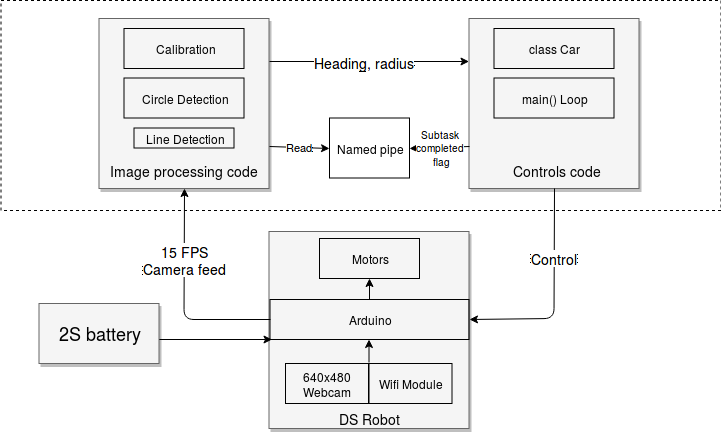
\includegraphics[width=0.9\columnwidth]{blockDiagram.png}
\end{center}
\end{figure}

\subsection{Usage}
The code can be used on any of the nix-like systems. A usage for the code is as follows:
\begin{lstlisting}[language=bash,caption={usage}]
$ cd c++ && make && cd ..
$ python ballTracking.py | c++/bin/main 192.168.1.1 2001
\end{lstlisting}

\section{Image processing}
The three main steps here are: creating a binary color mask, finding contours and identifying where the center of a minimum enclosing circle around that contour is, and deciding when the robot should stop. 

\subsection{Masking}
\texttt{range-detector.py} provides a simple GUI to determine a color range we want to identify. We extended the code taken from imutils package to support LAB color space calibration. The choice of this particular color space was motivated by our desire to have an algorithm that is robust to changes in scene lighting. The LAB space encodes intensity (luminance) and color (chrominance) in independent channels (L for luminance, A for green-red range and B for blue-yellow). In the GUI, the user can drag sliders to set lower and upper limits for different color space components. The results are updated in the form of a binary mask, where the identified range will result in pixels having value of 1, while others have a value of 0. 
\newline
Masking the image in \texttt{ballTracking.py} means applying \texttt{cv2.inRange()} to the image, with lower and upper limits previously determined by calibration as arguments. Further, we want to remove small blobs using \texttt{cv2.erode()} and \texttt{cv2.dilate()} functions. 

\subsection{Finding a ball center}
The main heavy lifting is done by \texttt{cv2.findContours()} method, which approximates main contours in the binary image. Each of the identified contours has a corresponding area, which means that the contour with maximal area is likely the one we are looking for. Now, we expect that the dominant contour in the image will be a circle, which means that we can fit the contour with a circle -- OpenCV conveniently has \texttt{cv2.minEnclosingCircle()} method. Further, we can find the circle center by computing moments (\texttt{cv2.moments()} that uses Green formula, as per OpenCV documentation) of the image enclosed by the contour. The moments give area and centroid information, where in our case the centroid corresponds to the circle center. In case the resulting circle radius is less than a threshold (set to 10 pixels in our case), we reject the found contours.

\subsection{Stop condition}
In case we were following a leader, we stop if the radius of the detected circle is greater than $0.75 \times $ \texttt{halfFrameWidth}. Otherwise, the relevant parameter is y-coordinate of the circle center, meaning that the ball is either beneath us or right in front of us. 

\section{Controls}
The controls code is located at \texttt{c++/main.cpp} in the repository.
\subsection{Communication Protocol}
For every frame that is analyzed, it is necessary to get a heading for the direction in which to go for the ball. This is accomplished by receiving two integers---displacement from the middle of the frame to the center of the ball (negative if the center of the ball is on the left half of the frame, positive otherwise) and radius of the ball---from the image processing program. The general protocol sequence works as follows:
\begin{itemize}
\item Start.
\item Read the \texttt{halfFrameWidth}. This will be important afterwards to scale left and right wheels speed while correcting direction on the go for the robot if the target moves. Operate on the received values.
\item In a loop, read the \texttt{degree} and \texttt{radius} values, and operate on them.
\end{itemize}

\subsection{class Car}
The \texttt{class Car\{\}} is the model for the robot. The initializer for the class opens a socket to connect to the robot at the ip and port provided as \texttt{argv} while starting the program. The initial speed of the robot is set to \texttt{SEARCH\_SPEED} defined in the header. The class provides the function \texttt{move()} that accepts macros \texttt{MOV\_FWD, MOV\_BWD, MOV\_LEFT,} and \texttt{MOV\_RIGHT} to mov in the respective direction.Other available functions are \texttt{setSpeed(), setRightSpeed(), setLeftSpeed(),} and \texttt{stop()}.
\subsection{main() loop}
Once \texttt{halfFrameWidth} has been established as per the communication protocol, the main control loop is triggered. The loop operates as follows:
\begin{itemize}
\item Read \texttt{degree} and \texttt{radius}
\item If \texttt{degree == halfFrameWidth} then no ball is within the frame. Set speed to \texttt{SEARCH\_SPEED}. Turn around to locate a ball. If a ball was previously spotted in then missed, the robot turns in the direction in which the ball was disappearing in the earlier frames. The remembering operation is accomplised by setting \texttt{moving\_fwd, moving\_left,} and \texttt{moving\_right} variables appropriately whenever a \texttt{degree} is received.
\item If \texttt{degree == -halfFrameWidth} then the robot has approached the ball and is close enough. Stop.
\item If \texttt{degree} is within $\pm$\texttt{CONCESSION} of \texttt{halfFrameWidth}, keep moving in a straight line. This reduces the jerky motion that would come from having constant adjustment with no concession margin. Additionally, the robot slows down as it gets closer to the ball. This is done by calibrating distance from the ball based on radius of the ball in the frame.
\item Else, map the degree received to a value between \texttt{CRUISE\_SPEED} (default is $40$) and \texttt{FULL\_SPEED} $(100)$. Set the relevant side to the faster speed in order to turn.
\end{itemize}

\subsection{Trajectory Following}
For this challenge, we had to make changes to our solution on the controls side. We decided to place 5 differently colored ping-pong balls on the trajectory (see Fig \ref{trajectory}) and follow them one by one. Ping-pong balls were chosen for this part since we were able to leave them between the wheels and pass over them on our way to the end.
\begin{figure}[h]
\caption{Trajectory challenge setup}\label{trajectory}
\begin{center}
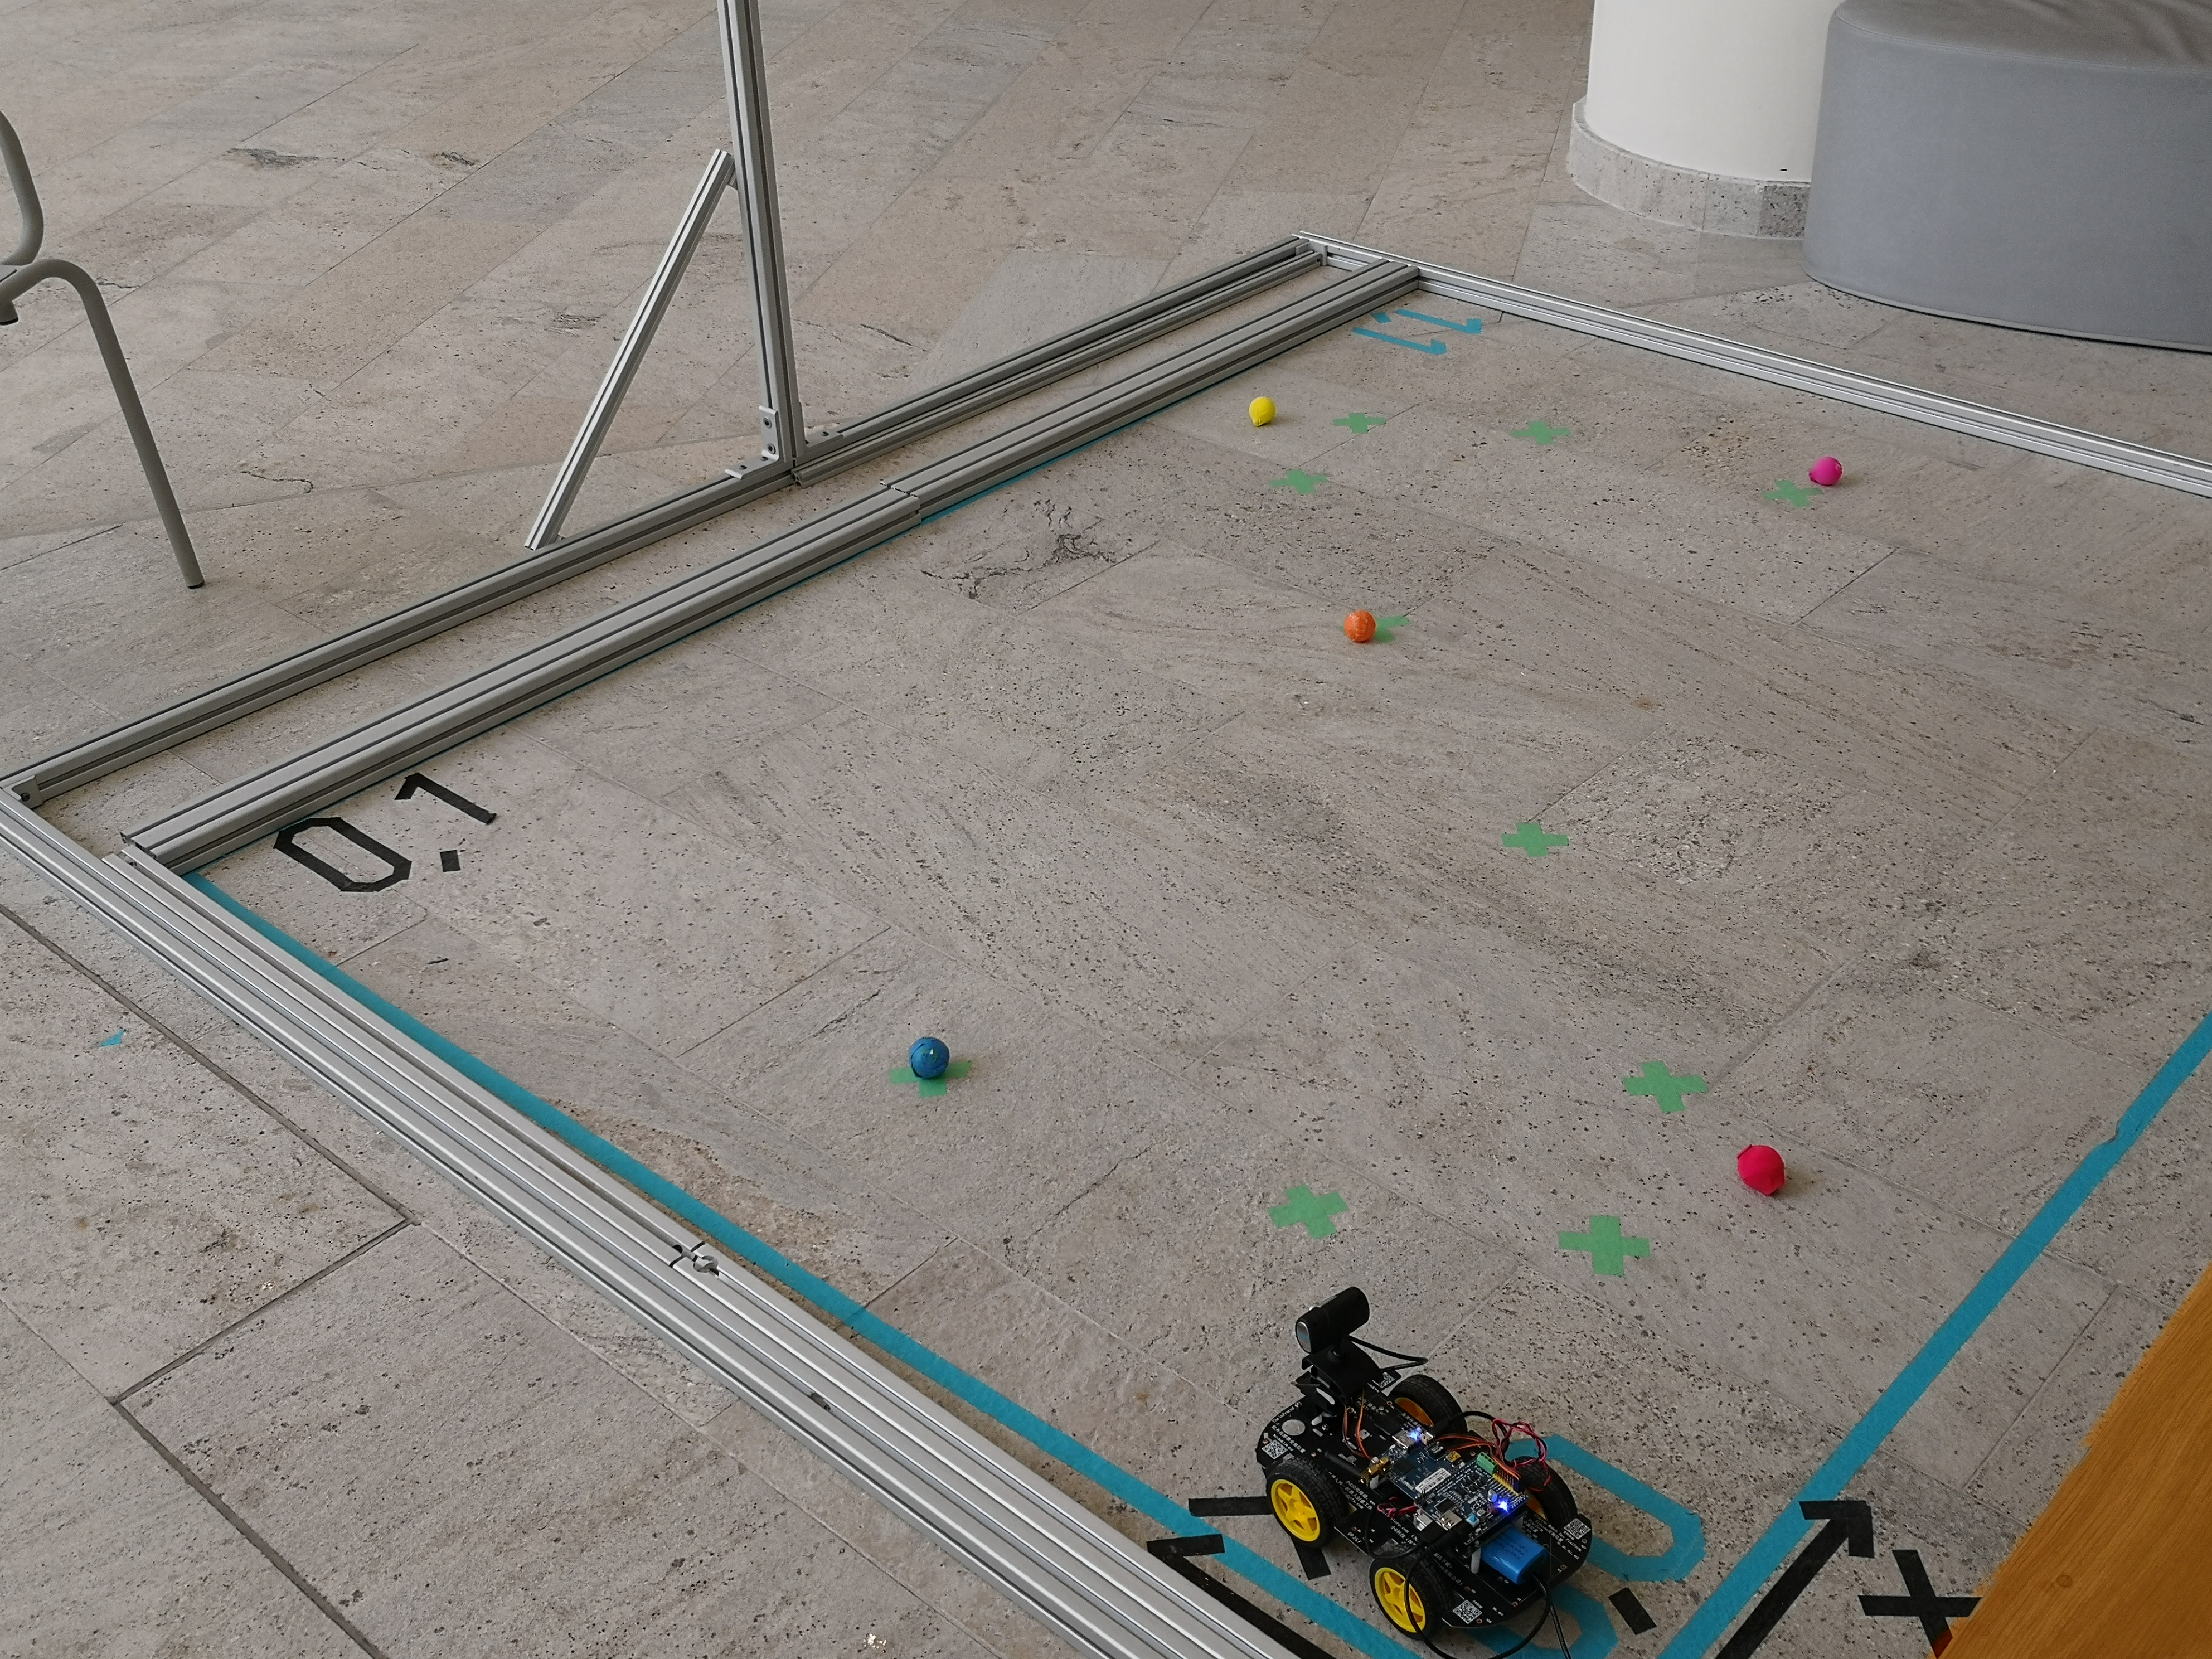
\includegraphics[width=0.9\columnwidth]{trajectory.jpg}
\end{center}
\end{figure}
\newline
Because of this setup, we needed to inform the image processing module about having reached one of the balls from the controls code. For image processing, this means that the LAB color mask is changed. Because up to this point, the communication was only going in one direction, i.e. from the image processing to controls, we needed a different mechanism for the communication in the other direction. For this, we chose to use named pipes. In Unix systems, they are seen as "lightweight files", whose read/write is handled by the kernel and these operations are therefore faster than in traditional temporary files. As soon as the reader reads the content of the pipe, the named pipe can be closed until the next write. The pipe can be unlinked and therefore disappears when the program terminates. Since our image processing code was to read from the pipe, we show the following read listing in Python and the write listing in C++. The \texttt{os.O\_NONBLOCK} flag was important to ensure we do not block other code execution while we wait for data to be written to the pipe (in this case, we just print ellipsis).  

\begin{lstlisting}[language=Python, caption=creating and reading from pipe]
import os
import posix

FIFO = 'mypipe'
# For the sample code, it suffices we open the pipe with maximum permissions
os.mkfifo(FIFO, 0o777)

def readPipe():
    while True:
        try:
            p = os.open(FIFO, os.O_RDONLY | os.O_NONBLOCK)
            input = os.read(p, 1) # we expect only 1 byte
        except:
            continue
        
        # Break as soon as we read successfully 
        if input:
            break

        os.close(p)
        print('...')

readPipe()
os.unlink(FIFO)
\end{lstlisting}

\begin{lstlisting}[language=C++, caption=write to pipe]
#include <iostream>
#include <fcntl.h>
#include <unistd.h>
#include <stdio.h>
#include <string.h>

int main(){
    char FIFO[] = "../mypipe";
    int fd;
    while (1) {
        fd = open(FIFO, O_WRONLY);
        write(fd, "1", 1);
        close(fd);
    }
    return 0;
}

\end{lstlisting}

Because of the specific requirements of the trajectory, some custom tweaks were made to controls code.
\begin{itemize}
\item In terms of protocol, we keep track of the first time we see the ball. In the subsequent frames, if the ball is not seen anymore, a flag is sent through the named pipe to the image processing code to indicate that the ball that was being searched for was reached. The image processing code then starts tracking the ball of the next color.
\item In terms of the direction adjustment, because we had a predefined track in the requirements, corresponding directions to look for the next ball was predefined in the code.
\end{itemize}

\section{Results}
The overall results were up to the standards we set at the beginning of the work. The demo shows that our solution is robust to different lighting conditions; we turn without stopping and the feedback continuously and seamlessly improves our motion; the small ball tracking and switching for the trajectory following also showed excellent results. In the table \ref{times}, it can be seen that from the first to the last point on the trajectory, it takes us 9.09s. The precision was difficult to measure, as we do not keep track of our absolute coordinate space position. Instead, the video testifies that we only miss the second to last point on the trajectory by a few centimeters; otherwise, we go through each of the points almost perfectly. Our results were highly replicable and not particularly susceptible to noise.

\begin{table}
\begin{center}
\caption{Times for different trajectory points} \label{times}
\begin{tabular}{| c | c |}
\hline
time(s) & x, y \\
\hline
0.00 & 0.15, 0.50 \\
\hline
0.85 & 0.17, 0.28 \\
\hline
0.97 & 0.23, 0.16 \\
\hline
3.09 & 0.32, 0.20 \\
\hline
4.04 & 0.44, 0.38 \\
\hline
5.06 & 0.56, 0.62 \\
\hline
5.96 & 0.68, 0.80 \\
\hline
6.09 & 0.77, 0.84 \\
\hline
8.88 & 0.83, 0.72 \\
\hline
9.09 & 0.85, 0.50 \\
\hline
\end{tabular}
\end{center}
\end{table}

\end{document}